\documentclass{article}
\usepackage{tikz}
\usepackage{datetime2}
\usepackage{fontspec}
\setmainfont{IBM Plex Mono}

\begin{document}

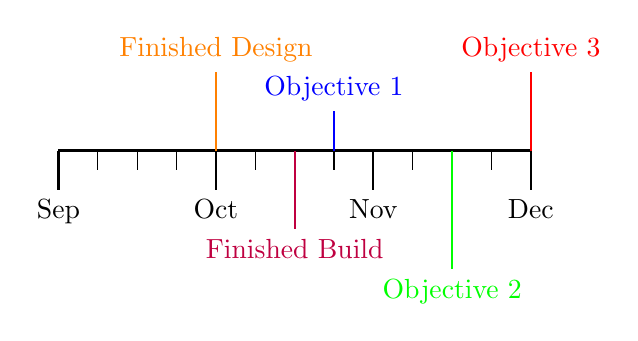
\begin{tikzpicture}
    % Draw the timeline line
    \draw[thick] (0,0) -- (6,0); % Timeline axis (8 units long)

    % Draw the months along the timeline (Sept to Dec)
    \foreach \x/\month in {0/Sep, 2/Oct, 4/Nov, 6/Dec} {
        \draw[thick] (\x,0) -- (\x,-0.5); % Major tick marks for each month
        \node[below] at (\x,-0.5) {\month}; % Month labels
    }

    % Add week tick marks (1 unit = 2 months, 4 weeks in each month, so 0.5 unit per week)
    \foreach \x in {0.5, 1, 1.5, 2.5, 3, 3.5, 4.5, 5, 5.5} {
        \draw[thin] (\x,0) -- (\x,-0.25); % Minor tick marks for weeks
    }

    % Milestones
    \draw[orange, thick] (2,0) -- (2,1) node[above] {Finished Design};
    \draw[purple, thick] (3,0) -- (3,-1) node[below] {Finished Build};
    \draw[blue, thick] (3.5,0) -- (3.5,0.5) node[above] {Objective 1};
    \draw[green, thick] (5,0) -- (5,-1.5) node[below] {Objective 2};
    \draw[red, thick] (6,0) -- (6,1) node[above] {Objective 3};
\end{tikzpicture}

\end{document}
